\documentclass[12pt]{article}

\usepackage[margin=0.5in]{geometry}
\usepackage{amsmath, amssymb}
\usepackage{hyperref}
\usepackage{tikz}
\renewcommand{\arraystretch}{1.6}

% Header pset untuk halaman pertama
\newcommand{\psetheader}[4]{%
  \noindent
  \begin{minipage}[t]{0.6\textwidth}
    #1\\
    #2\\
    #3
  \end{minipage}%
  \hfill
  \begin{minipage}[t]{0.35\textwidth}
    \raggedleft #4
  \end{minipage}

  \vspace{0.5\baselineskip}
  \hrule
  \vspace{1em}
}

\title{Matematika Dasar - Tugas 2}
\author{Anas Azhar \ FST - Matematika - 056413438 \ Universitas Terbuka}
\date{\today}

\begin{document}

\psetheader
  {\textit{Matematika Dasar} - Tugas 2}
  {Universitas Terbuka, FST - Matematika, 2025.1}
  {Anas Azhar (056413438)}
  {Minggu, 16 November 2025}

\section*{Soal 1}
Tentukan nilai $x$ yang memenuhi pertidaksamaan:
\[
6 < 4x - 2 \ge 2.
\]

\noindent Pertidaksamaan tersebut setara dengan dua pertidaksamaan:
\[
6 < 4x - 2 \quad \text{dan} \quad 4x - 2 \ge 2.
\]

\subsection*{Penyelesaian}
\noindent Selesaikan masing-masing:

1. 
\[
6 < 4x - 2
\]
\[
6 + 2 < 4x
\]
\[
8 < 4x \implies x > 2.
\]

2.
\[
4x - 2 \ge 2
\]
\[
4x \ge 4
\]
\[
x \ge 1.
\]

\noindent Gabungan syarat:
\[
x > 2 \quad \text{dan} \quad x \ge 1 \implies x > 2.
\]

\[
\boxed{x > 2}
\]

\section*{Soal 2}

Tentukan nilai $x$ yang memenuhi persamaan dan pertidaksamaan mutlak berikut:
\begin{enumerate}
    \item[(a)] $|4x + 18| = 2$
    \item[(b)] $|5x - 9| < 6$
\end{enumerate}

\section*{Penyelesaian}

\subsection*{a. Persamaan mutlak $|4x + 18| = 2$}

Persamaan mutlak memenuhi:
\[
|A| = k \iff A = k \text{ atau } A = -k.
\]

Maka:
\[
4x + 18 = 2 \quad \text{atau} \quad 4x + 18 = -2.
\]

Kasus pertama:
\[
4x + 18 = 2 \implies 4x = -16 \implies x = -4.
\]

Kasus kedua:
\[
4x + 18 = -2 \implies 4x = -20 \implies x = -5.
\]

\[
\boxed{x = -4 \text{ atau } x = -5}
\]

\subsection*{b. Pertidaksamaan mutlak $|5x - 9| < 6$}

Untuk pertidaksamaan mutlak:
\[
|A| < k \iff -k < A < k.
\]

Maka:
\[
-6 < 5x - 9 < 6.
\]

Tambahkan 9 pada semua ruas:
\[
3 < 5x < 15.
\]

Bagi semua ruas dengan 5:
\[
\boxed{\frac{3}{5} < x < 3}
\]

\subsection*{Garis Bilangan untuk Himpunan Penyelesaian}

\begin{center}
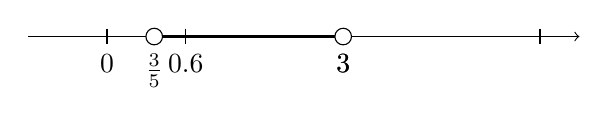
\begin{tikzpicture}[x=1cm, y=1cm]
    % Garis bilangan
    \draw[->] (-1,0) -- (6,0);

    % Titik penting
    \foreach \x/\label in {0/0, 1/0.6, 3/3, 5.5/{}}
        \draw (\x,0.1) -- (\x,-0.1) node[below] {\label};

    % Titik batas 3/5
    \draw (0.6,0.1) -- (0.6,-0.1) node[below] {$\frac{3}{5}$};

    % Titik batas 3
    \draw (3,0.1) -- (3,-0.1) node[below] {$3$};

    % Interval terbuka (3/5, 3)
    \draw[very thick] (0.6,0) -- (3,0);

    % Lingkaran kosong
    \draw[fill=white] (0.6,0) circle (3pt);
    \draw[fill=white] (3,0) circle (3pt);
\end{tikzpicture}
\end{center}

\section*{Soal 3}

Didefinisikan relasi pengurangan $(-)$ pada himpunan bilangan asli $\mathbb{N}$ sebagai berikut:
\[
\forall x,y \in \mathbb{N}, \quad x \mathcal{R} y \iff x - y \in \mathbb{N}.
\]
Selidiki dan tunjukkan apakah relasi $\mathcal{R}$ bersifat:
\begin{enumerate}
    \item Refleksif,
    \item Simetris,
    \item Transitif.
\end{enumerate}

\section*{Penyelesaian}

Kita gunakan $\mathbb{N} = \{1,2,3,\dots\}$ (tanpa nol), sehingga
\[
x \mathcal{R} y \iff x-y \in \mathbb{N} \iff x > y.
\]

\subsection*{a. Refleksif}

Suatu relasi $\mathcal{R}$ pada $\mathbb{N}$ dikatakan \emph{refleksif} jika
\[
\forall x \in \mathbb{N},\ (x,x) \in \mathcal{R},
\]
atau setara dengan $x \mathcal{R} x$ untuk semua $x$.

Perhatikan
\[
x \mathcal{R} x \iff x - x \in \mathbb{N} \iff 0 \in \mathbb{N}.
\]
Karena $0 \notin \mathbb{N}$ (bilangan asli dimulai dari 1), maka
\[
x \mathcal{R} x \text{ tidak berlaku untuk sembarang } x.
\]
Contoh: untuk $x=1$,
\[
1-1 = 0 \notin \mathbb{N},
\]
jadi $(1,1) \notin \mathcal{R}$.

Maka:
\[
\boxed{\mathcal{R} \text{ tidak refleksif.}}
\]

\subsection*{b. Simetris}

Relasi $\mathcal{R}$ dikatakan \emph{simetris} jika
\[
\forall x,y \in \mathbb{N},\ x \mathcal{R} y \implies y \mathcal{R} x.
\]

Ambil contoh $x=5$, $y=3$:
\[
5 \mathcal{R} 3 \iff 5-3 = 2 \in \mathbb{N} \quad (\text{benar}).
\]
Tetapi:
\[
3 \mathcal{R} 5 \iff 3-5 = -2 \in \mathbb{N} \quad (\text{salah}).
\]

Karena ada pasangan $(5,3) \in \mathcal{R}$ tetapi $(3,5) \notin \mathcal{R}$, maka:
\[
\boxed{\mathcal{R} \text{ tidak simetris.}}
\]

\subsection*{c. Transitif}

Relasi $\mathcal{R}$ dikatakan \emph{transitif} jika
\[
\forall x,y,z \in \mathbb{N},\ \big(x \mathcal{R} y \land y \mathcal{R} z\big) \implies x \mathcal{R} z.
\]

Misalkan
\[
x \mathcal{R} y \text{ dan } y \mathcal{R} z.
\]
Ini berarti
\[
x - y \in \mathbb{N} \quad \text{dan} \quad y - z \in \mathbb{N},
\]
atau setara dengan
\[
x > y \quad \text{dan} \quad y > z.
\]
Dari sifat ketidaksamaan pada bilangan asli, diperoleh:
\[
x > y > z \implies x > z.
\]
Karena $x>z$, maka
\[
x - z \in \mathbb{N} \implies x \mathcal{R} z.
\]

Jadi sifat transitif terpenuhi:
\[
\boxed{\mathcal{R} \text{ transitif.}}
\]

\section*{Kesimpulan}
Relasi $\mathcal{R}$ pada $\mathbb{N}$ yang didefinisikan oleh
\(
x \mathcal{R} y \iff x-y \in \mathbb{N}
\)
adalah:
\[
\boxed{\text{tidak refleksif, tidak simetris, tetapi transitif.}}
\]

\end{document}